\section[تمرین دوم - سؤال دوم: بیشینه درست‌نمایی (MLE) با توزیع لاپلاس]
{\faProjectDiagram\ \ تمرین دوم ـ سؤال دوم: تخمین بیشینه درست‌نمایی (\lr{MLE}) و رگرسیون لاپلاس}

\begin{stepbox}

\field{هدف و معرفی مسئله}{
هدف این بخش، پیاده‌سازی روش **تخمین بیشینه درست‌نمایی (\lr{Maximum Likelihood Estimation - MLE})** بر روی داده‌های زمان فوران آتشفشان (\lr{Q2.csv}) با فرض تابع توزیع لاپلاس (\lr{Laplace Distribution}) و مقایسه عملکرد آن با رگرسیون خطی معمولی (\lr{OLS / $L_2$}) می‌باشد.

در بسیاری از مسائل دنیای واقعی، داده‌ها ممکن است حاوی نقاط پرت (\lr{Outliers}) باشند یا توزیع خطا غیرگوسی باشد. تابع توزیع لاپلاس به دلیل استفاده از قدر مطلق خطاها در لوگ-درست‌نمایی، مقاومت به مراتب بالاتری در برابر داده‌های پرت دارد.
}

\field{تعریف ریاضی لگاریتم منفی درست‌نمایی (NLL)}{
فرمول منفی لگاریتم درست‌نمایی (\lr{Negative Log-Likelihood}) برای $n$ نمونه مستقل با توزیع لاپلاس به صورت زیر تعریف می‌شود:

\[
\ell(y_1, y_2, \dots, y_n; \mu, \lambda) = -\sum_{i=1}^{n} \left( -\log(2\lambda) - \frac{|y_i - \mu|}{\lambda} \right)
\]

در مدل رگرسیون غیرخطی این تمرین، میانگین توزیع به صورت نمایی وابسته به ویژگی‌ها در نظر گرفته شد:

\[
\mu = \exp(\mathbf{X}\mathbf{b})
\]

جهت بهینه‌سازی و یافتن ضرایب $\mathbf{b}$، از الگوریتم بهینه‌سازی \lr{Powell} درون تابع \lr{scipy.optimize.minimize} استفاده گردید.
}

\field{برازش مدل لاپلاس بر روی داده‌های واقعی}{
پس از تعریف توابع `laplaceRegNegLogLikelihood` و `modelFit`، ضرایب بهینه $\mathbf{b}$ برای داده‌های مجموعه \lr{Q2.csv} استخراج شده و منحنی پیش‌بینی برای داده‌های جدید $x \in [0, 6]$ ترسیم گردید.

\vspace{0.4cm}

\begin{center}
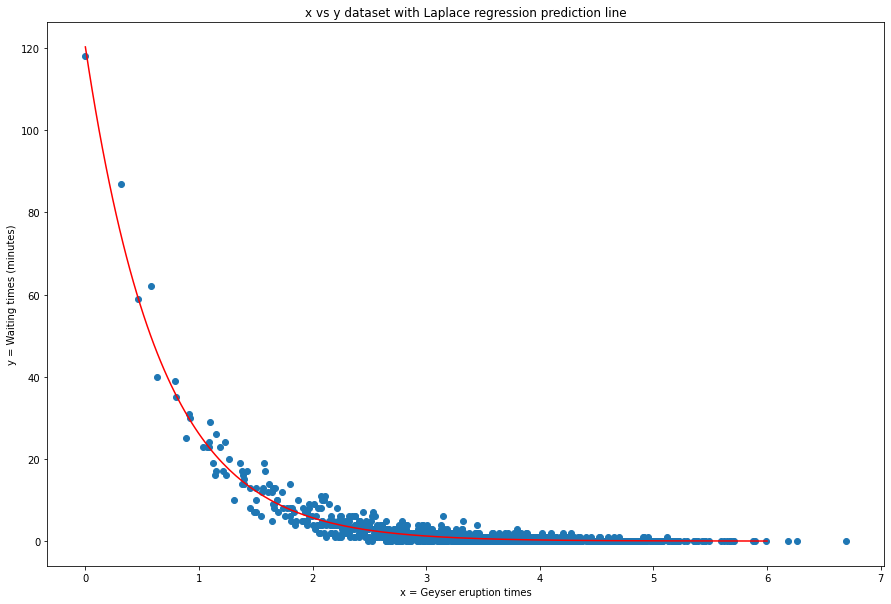
\includegraphics[width=.78\textwidth]{images/laplace_fit.png}
\captionof{figure}{برازش رگرسیون لاپلاس ($\mu = \exp(\mathbf{X}\mathbf{b})$) بر روی داده‌های زمان فوران و انتظار}
\label{fig:laplace_fit}
\end{center}
}

\field{برازش رگرسیون خطی معمولی (OLS / $L_2$) و مقایسه}{
در ادامه، مدل رگرسیون خطی معمولی با فرض توزیع خطا به صورت گوسی (کمترین مربعات) بر روی همان داده‌ها برازش داده شد.

\vspace{0.4cm}

\begin{center}
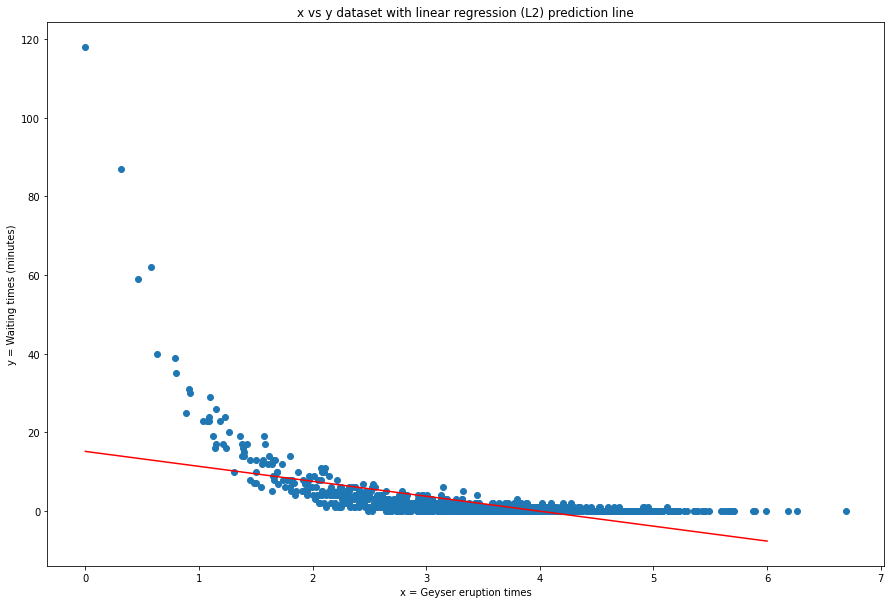
\includegraphics[width=.78\textwidth]{images/ols_fit.png}
\captionof{figure}{برازش رگرسیون خطی معمولی (\lr{OLS / $L_2$}) بر روی مجموعه داده}
\label{fig:ols_fit}
\end{center}
}

\field{تحلیل و پاسخ به خواسته سوال (چرا رگرسیون خطی دچار مشکل است؟)}{
با مقایسه دو نمودار فوق، نتایج تحلیلی زیر استخراج گردید:

\begin{itemize}
\item **ضعف رگرسیون خطی $L_2$ در برابر داده‌های پرت:**
در الگوریتم $L_2$، خطای هر نقطه به توان ۲ می‌رسد ($|y_i - \hat{y}_i|^2$). نقاط پرتی که مقدار $y$ آن‌ها بسیار بزرگ است، جریمه فوق‌العاده شدیدی به تابع هزینه تحمیل می‌کنند. این امر باعث می‌شود که خط رگرسیون به شدت به سمت نقاط پرت منحرف شده و توانایی خود را در پیش‌بینی دقیق تنه اصلی داده‌ها از دست بدهد (\lr{Underfitting} روی داده‌های اصلی).

\item **مزیت رگرسیون لاپلاس ($L_1$):**
توزیع لاپلاس از قدر مطلق خطاها ($|y_i - \hat{y}_i|$) استفاده می‌کند. این ویژگی باعث می‌شود که تاثیر نقاط پرت به صورت خطی رشد کند نه نمایی؛ در نتیجه مدل لاپلاس نسبت به نقاط پرت استوار (\lr{Robust}) بوده و رفتار واقعی روندهای نمایی در داده‌ها را بسیار دقیق‌تر مدل‌سازی می‌کند.
\end{itemize}
}

\field{جمع‌بندی}{
در این تمرین، با پیاده‌سازی دستی تابع درست‌نمایی لاپلاس و بهینه‌سازی آن، نشان داده شد که انتخاب تابع توزیع مناسب متناسب با ماهیت داده‌ها اهمیت بالایی دارد. رگرسیون لاپلاس به دلیل استواری در برابر داده‌های پرت (\lr{Outlier Robustness}) و فرم نمایی $\mu = \exp(\mathbf{X}\mathbf{b})$، عملکرد بسیار برتری نسبت به رگرسیون خطی معمولی ارائه داد.
}

\end{stepbox}